\documentclass[conference]{IEEEtran}
\usepackage{config/ieee-paper}
\usepackage{lipsum}
\hyphenation{
    % A
    %
    % B
    %
    % C
    %
    % D
    %
    % E
    %
    % F
    %
    % G
    %
    % H
    %
    % I
    % 
    % J
    %
    % K
    %
    % L
    %
    % M
    %
    % N
    %
    % O
    %
    % P
    %
    % Q
    %
    % R
    %
    % S
    %
    % T
    % 
    % U
    %
    % V
    %
    % W
    %
    % X
    %
    % Y
    % 
    % Z
    %
}

% Adding references to the document
\addbibresource{IEEEabrv.bib}
\addbibresource{references.bib}

\IEEEoverridecommandlockouts{}
% The preceding line is only needed to identify funding in the first footnote. If that is unneeded, please comment it out.
\begin{document}

\title{CSC730: Assignment 6\\Measuring Performance – ROC and PR Curves

}

\author{\IEEEauthorblockN{Kristophor Ray Jensen}
    \IEEEauthorblockA{\textit{Electrical Engineering and Computer Science} \\
        \textit{South Dakota School of Mines and Technology}\\
        Rapid City, United States \\
        0009-0001-7344-349X}

}

\maketitle

%\begin{abstract}
\lipsum[1]
\end{abstract}

\begin{IEEEkeywords}
    ADBench, Anomaly Detection, Skewed MNIST, Assignment 5, CSC730
\end{IEEEkeywords}


\section{Introduction}
For assignment 5 we are tasked to learn about ADBench, a so-called anomaly detection toolset. 
This toolset is a compilation of 57 datasets and 30 anomaly detection algorithms. These algorithms
can be classified as supervised, semi-supervised, and unsupervised. ADBench was
presented in a paper by Han et al. in 2022 and at the 36th Conference on Neural 
Information Processing Systems (NeurIPS 2022). The paper is titled "AD-Bench: A Benchmark for Anomaly Detection in High-Dimensional Data"\ \cite{han2022adbench}.

The assignement objectives are listed in the next section. One of the common themes of this assignment is the re-utilization of the 'skewed$\_$MNIST` dataset.
In this report we will discuss the installation of ADBench, the application of two algorithms to the `skewed$\_$MNIST` dataset, and the characterization of the results.


\section{Homework Objectives}

The specific objectives of this assignment are as follows \cite{assignment6}:
\begin{itemize}
    \item Get the MNIST and MNIST-C dataset.
    \item Select 3 different types of image corruption (e.g., canny edges) from MNIST-C.
    \item Create mixed datasets for training and test using the original MNIST and corrupted images at a 100/1 ratio for each corruption type.
    \item Create a probability density-based anomaly detector.
    \item Using a range of probability thresholds, create the corresponding ROC and precision-recall curves.
\end{itemize}


\section{Methodology}
\subsection{Data Preparation}
The first step in the assignment was to download the MNIST and MNIST-C datasets. 
We then selected three different types of image corruptions from the MNIST-C dataset.
For each type of corruption, we created a mixed dataset for training and testing. 
This mixed dataset combined the original MNIST images with the corrupted images at a ratio of 100/1. 
This resulted in a dataset that was predominantly composed of normal images, with a small proportion of anomalous (i.e., corrupted) images.\par

Three mixed datasets were created using three seperate selections of corruptions.
The sets of corruptions, chosen randomly, were: "canny, dotted, stripe", "shear, canny, spatter", and "stripe, motion, scale".

\subsection{Visual Review}
We visually reviewed the mixed datasets to ensure that the normal data, fig.~\ref{fig1}, and anomalous images fig(s).~\ref{fig2} through fig(s).~\ref{fig8} were correctly labeled. This step was important to ensure that the anomaly detector was trained on the correct data.\par
\begin{figure}[htbp]
    \centerline{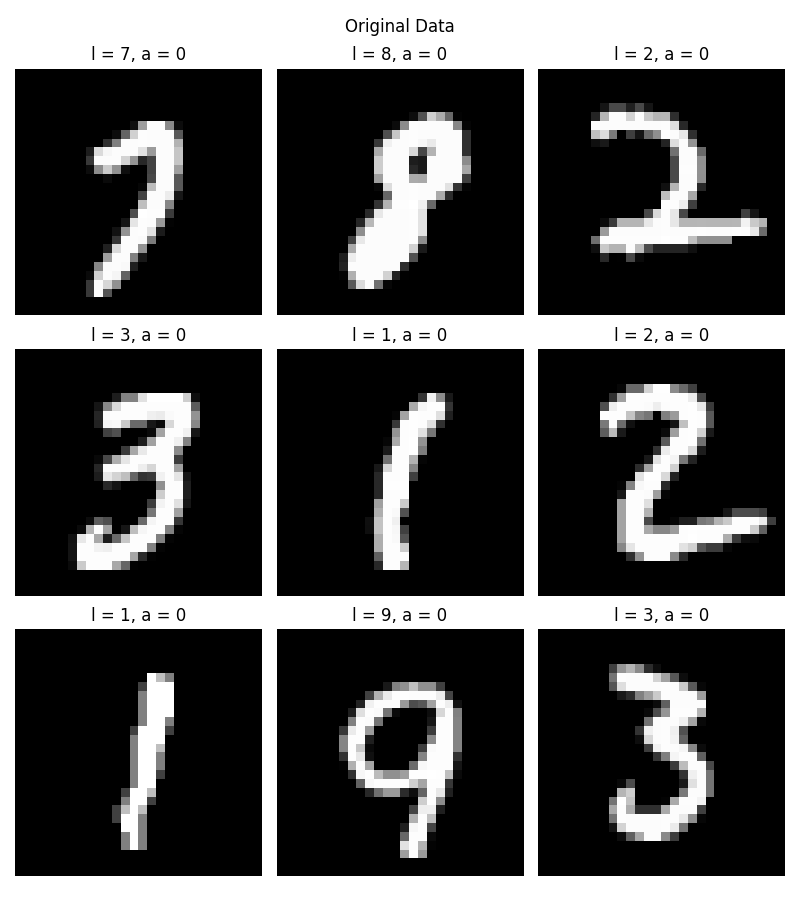
\includegraphics[width=0.5\textwidth]{resources/original_data.png}}
    \caption{Original MNIST data}\label{fig1}
\end{figure}

\begin{figure}[htbp]
    \centerline{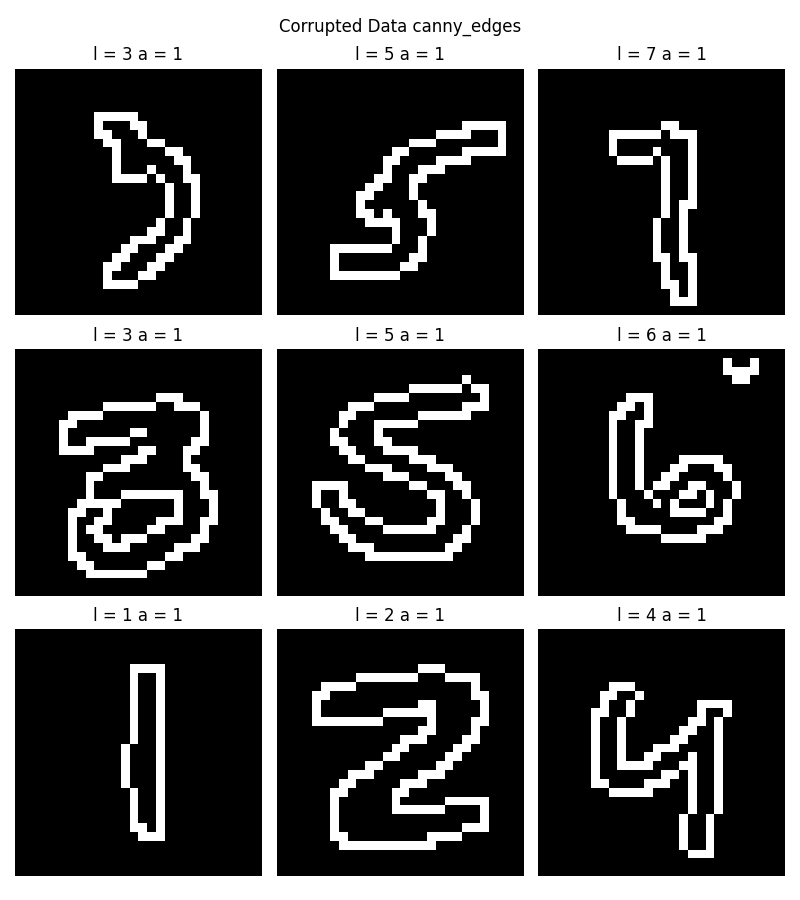
\includegraphics[width=0.5\textwidth]{resources/corrupted_data_canny_edges.png}}
    \caption{MNIST-C, canny edges}\label{fig2}
\end{figure}

\begin{figure}[htbp]
    \centerline{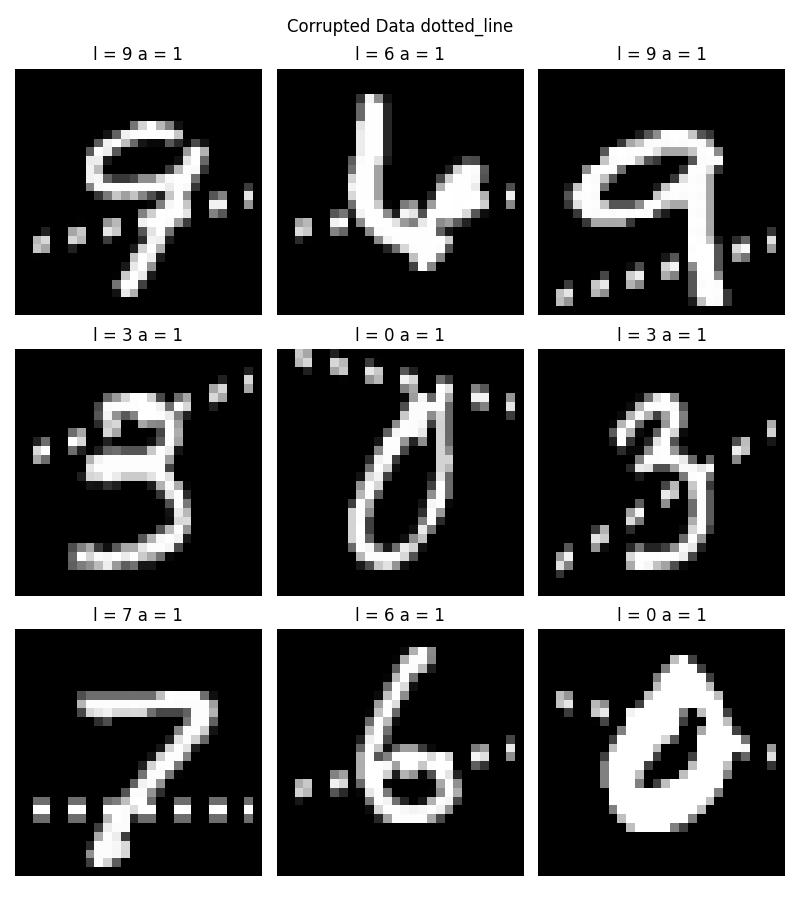
\includegraphics[width=0.5\textwidth]{resources/corrupted_data_dotted_line.png}}
    \caption{MNIST-C, dotted line}\label{fig3}
\end{figure}

\begin{figure}[htbp]
    \centerline{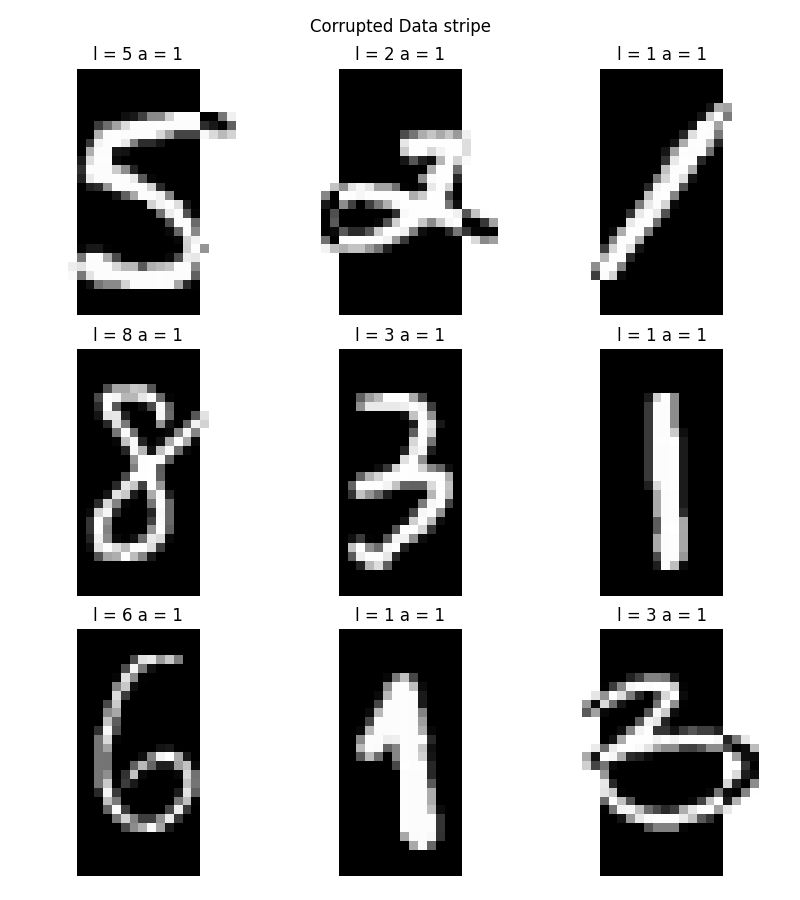
\includegraphics[width=0.5\textwidth]{resources/corrupted_data_stripe.png}}
    \caption{MNIST-C, stripe}\label{fig4}
\end{figure}

\begin{figure}[htbp]
    \centerline{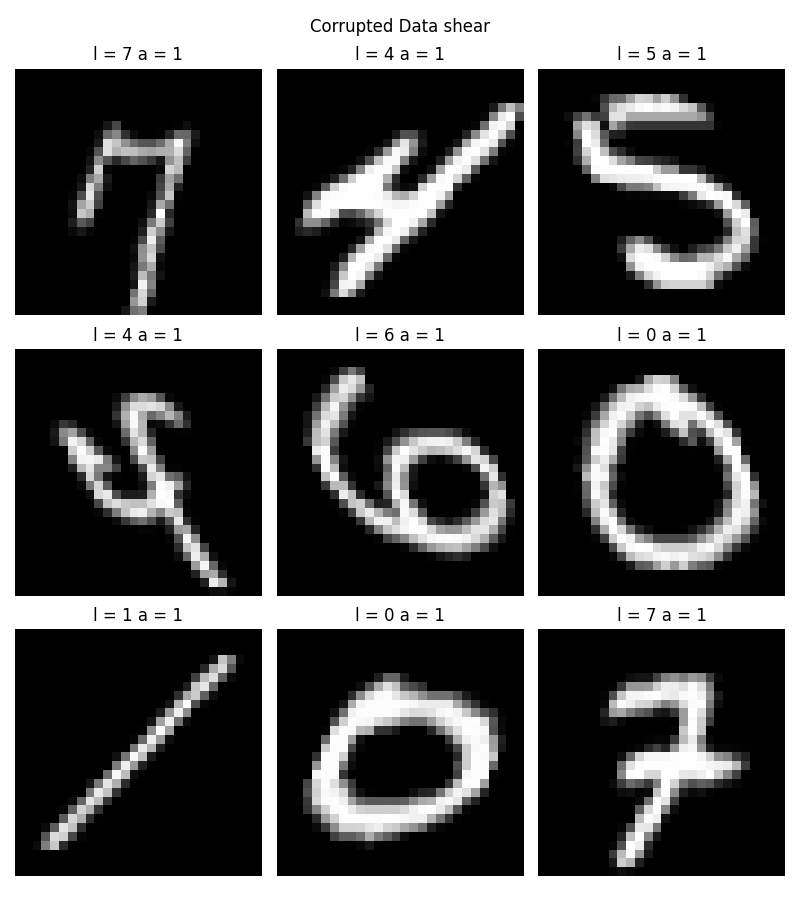
\includegraphics[width=0.5\textwidth]{resources/corrupted_data_shear.png}}
    \caption{MNIST-C, shear}\label{fig5}
\end{figure}

\begin{figure}[htbp]
    \centerline{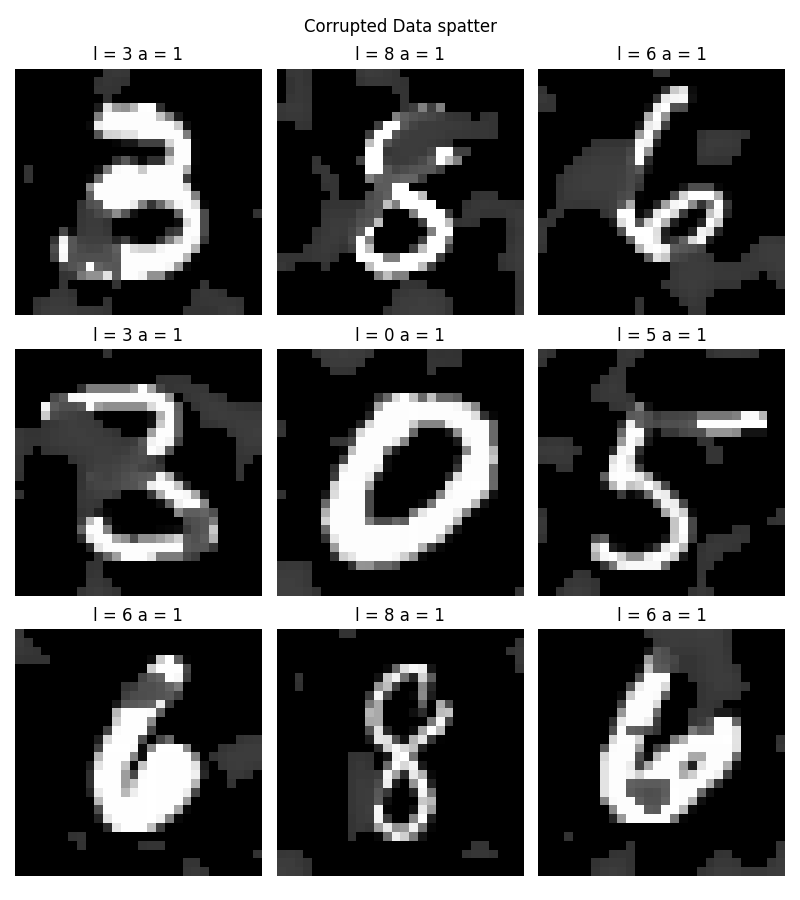
\includegraphics[width=0.5\textwidth]{resources/corrupted_data_spatter.png}}
    \caption{MNIST-C, spatter}\label{fig6}
\end{figure}

\begin{figure}[htbp]
    \centerline{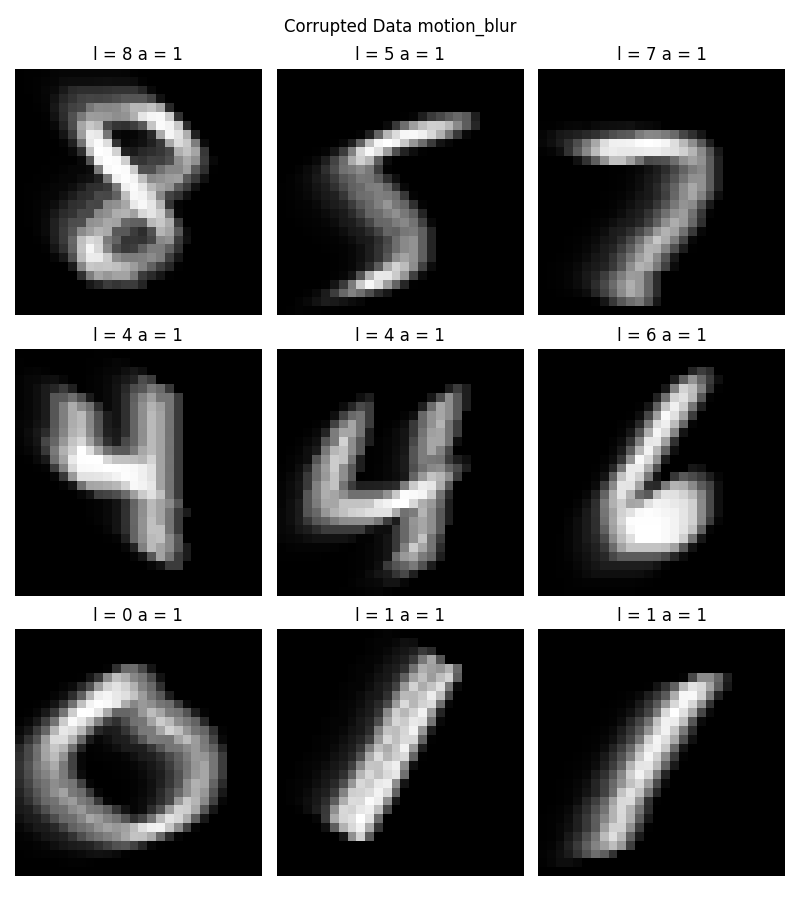
\includegraphics[width=0.5\textwidth]{resources/corrupted_data_motion_blur.png}}
    \caption{MNIST-C, motion blur}\label{fig7}
\end{figure}

\begin{figure}[htbp]
    \centerline{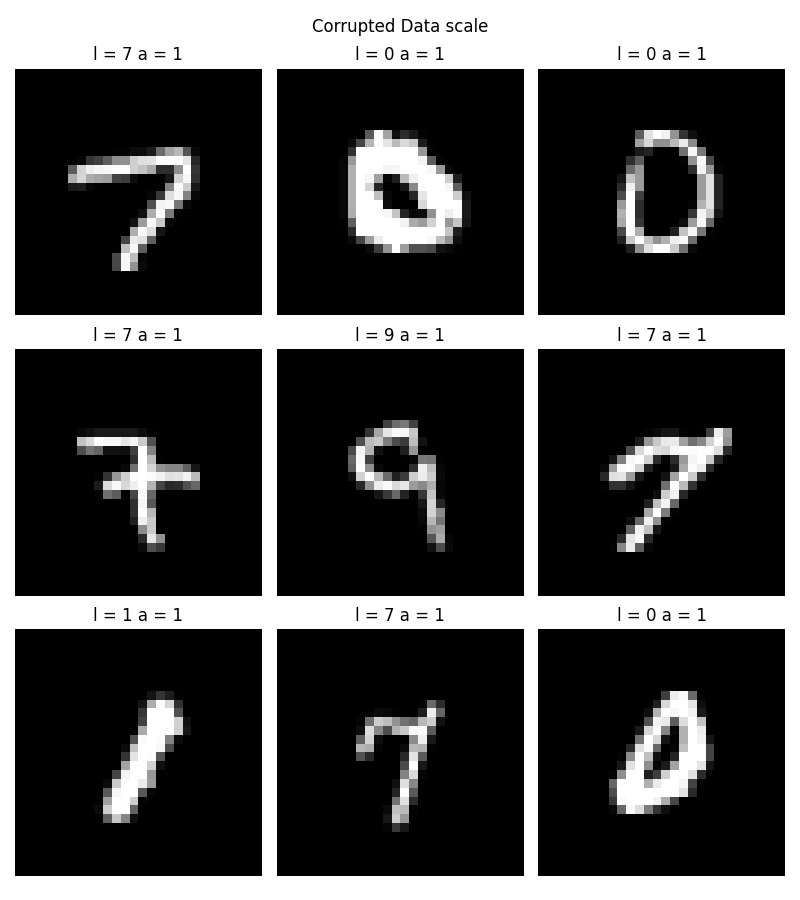
\includegraphics[width=0.5\textwidth]{resources/corrupted_data_scale.png}}
    \caption{MNIST-C, scale}\label{fig8}   
\end{figure}


\subsection{Anomaly Detection}
We implemented a probability density-based anomaly detector using the implementation from scikit-learn of K-Nearest Neighbors (KNN) and Random Forest(RF). 
This is a supervised learning algorithm where labels of anomaly and normal data are used to train the model.
The anomaly label is 1 for anomalous data and 0 for nominal data.\par

\subsection{Performance Evaluation}
We evaluated the performance of the anomaly detector using ROC and PR curves. 
The ROC curve plots the true positive rate against the false positive rate at different probability thresholds.
A true positive is an instance where the model correctly predicts the positive class, while a false positive is an instance where the model incorrectly predicts the positive class.\par
The PR curve plots the precision against the recall at different probability thresholds. 
Precision is the ratio of true positives to the sum of true positives and false positives, while recall is the ratio of true positives to the sum of true positives and false negatives.\cite{precision_recall_wiki}\par
These curves provide a visual representation of the trade-off between true positives and false positives, and between precision and recall, respectively.\par









\section{Results}
We ran three data trials: “canny, dotted, stripe”, “shear, canny, spatter”, and “stripe, motion, scale”. For each trial, we applied the KNN and the RF classifiers from the scikit-learn library. The KNN was executed from k=3 to k=10000, and the RF was fit with estimators of 3, 10, and 30.

The KNN performance was heavily sensitive to the data selected, whereas the RF was not so sensitive. In general, the KNN had poor performance, while the RF did a very good job detecting the anomalies.

\begin{figure}[htbp]
    \centerline{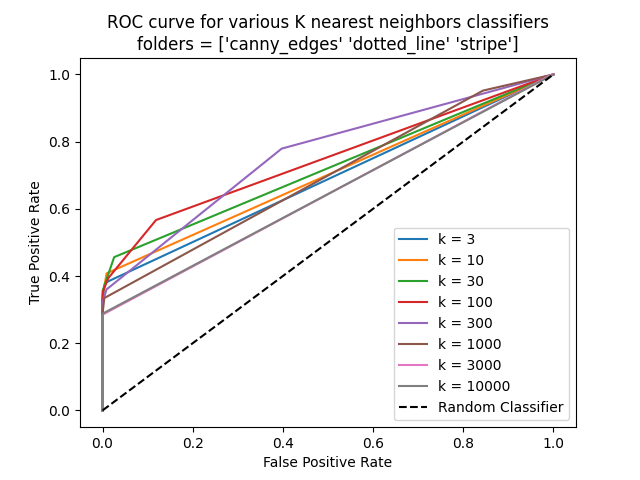
\includegraphics[width=0.5\textwidth]{resources/roc_curve_knn_canny_edges_dotted_line_stripe.png}}    
    \caption{ROC Curve for KNN: with canny edges, dotted lines and striped}\label{fig9}
\end{figure}

\begin{figure}[htbp]
    \centerline{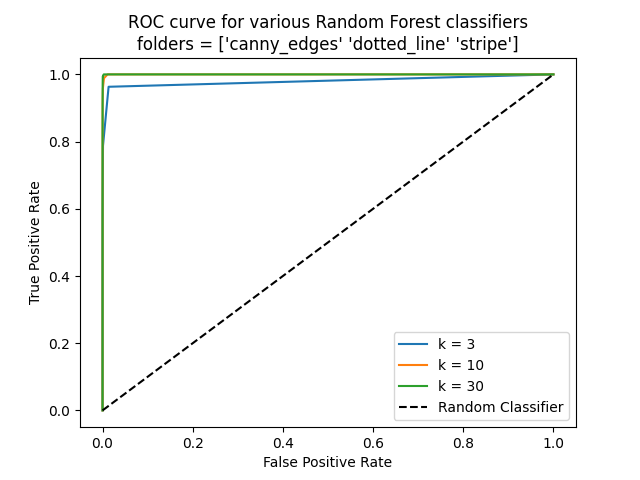
\includegraphics[width=0.5\textwidth]{resources/roc_curve_rf_canny_edges_dotted_line_stripe.png}}    
    \caption{ROC Curve for RF: with canny edges, dotted lines and striped}\label{fig10}
\end{figure}

\begin{figure}[htbp]
    \centerline{\includegraphics[width=0.5\textwidth]{resources/precision_recall_knn_canny_edges_dotted_line_stripe.png}}    
    \caption{PR Curve for KNN: with canny edges, dotted lines and striped}\label{fig11}
\end{figure}

\begin{figure}[htbp]
    \centerline{\includegraphics[width=0.5\textwidth]{resources/precision_recall_rf_canny_edges_dotted_line_stripe.png}}    
    \caption{PR Curve for RF: with canny edges, dotted lines and striped}\label{fig12}
\end{figure}

\begin{figure}[htbp]
    \centerline{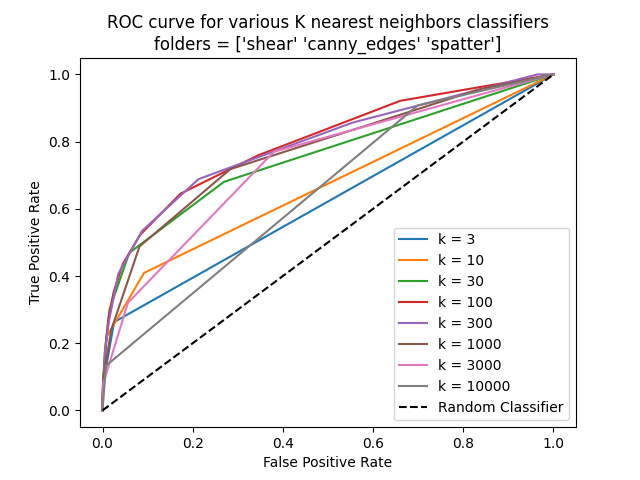
\includegraphics[width=0.5\textwidth]{resources/roc_curve_knn_shear_canny_edges_spatter.png}}    
    \caption{ROC Curve for KNN: with shear, canny edges, and spatter}\label{fig13}
\end{figure}

\begin{figure}[htbp]
    \centerline{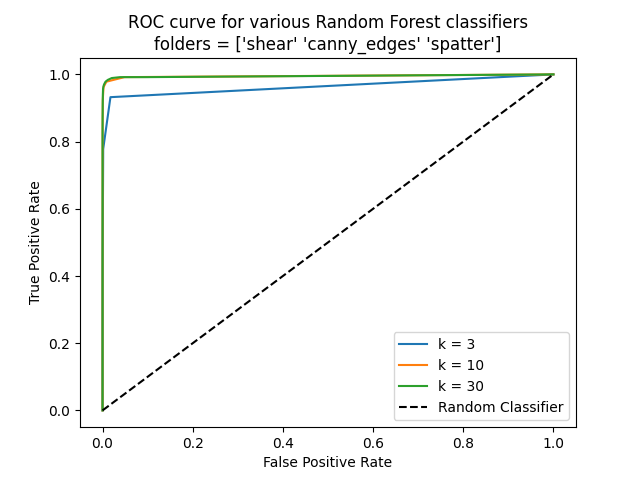
\includegraphics[width=0.5\textwidth]{resources/roc_curve_rf_shear_canny_edges_spatter.png}}    
    \caption{ROC Curve for RF: with shear, canny edges, and spatter}\label{fig14}
\end{figure}

\begin{figure}[htbp]
    \centerline{\includegraphics[width=0.5\textwidth]{resources/precision_recall_knn_shear_canny_edges_spatter.png}}    
    \caption{PR Curve for KNN: with shear, canny edges, and spatter}\label{fig15}
\end{figure}

\begin{figure}[htbp]
    \centerline{\includegraphics[width=0.5\textwidth]{resources/precision_recall_rf_shear_canny_edges_spatter.png}}    
    \caption{PR Curve for RF: with shear, canny edges, and spatter}\label{fig16}
\end{figure}

\begin{figure}[htbp]
    \centerline{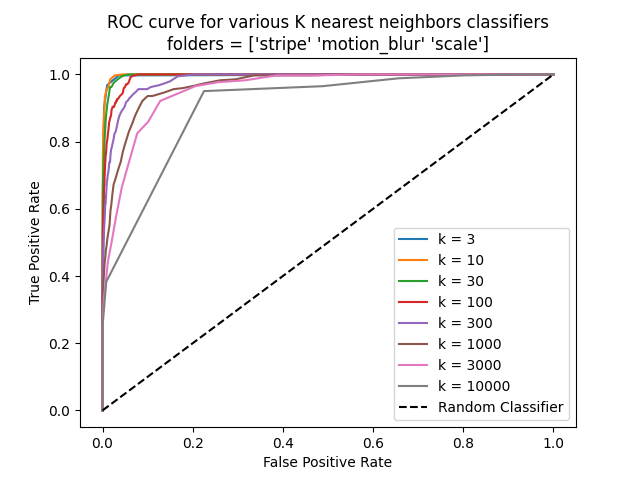
\includegraphics[width=0.5\textwidth]{resources/roc_curve_knn_stripe_motion_blur_scale.png}}    
    \caption{ROC Curve for KNN: with striped, motion blur, and scale}\label{fig17}
\end{figure}

\begin{figure}[htbp]
    \centerline{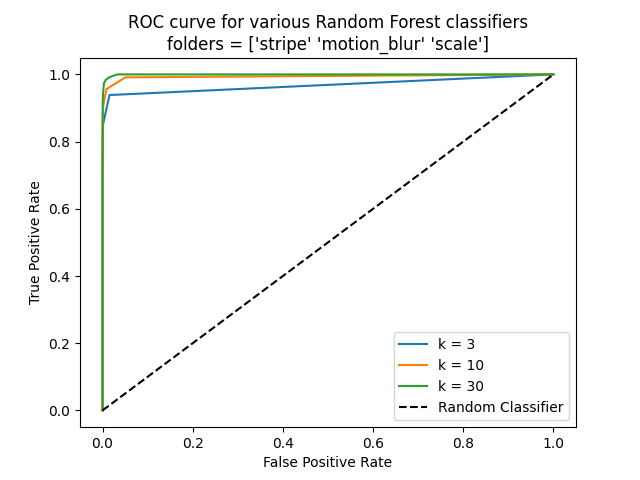
\includegraphics[width=0.5\textwidth]{resources/roc_curve_rf_stripe_motion_blur_scale.png}}    
    \caption{ROC Curve for RF: with striped, motion blur, and scale}\label{fig18}
\end{figure}

\begin{figure}[htbp]
    \centerline{\includegraphics[width=0.5\textwidth]{resources/precision_recall_knn_stripe_motion_blur_scale.png}}    
    \caption{PR Curve for KNN: with striped, motion blur, and scale}\label{fig19}
\end{figure}

\begin{figure}[htbp]
    \centerline{\includegraphics[width=0.5\textwidth]{resources/precision_recall_rf_stripe_motion_blur_scale.png}}    
    \caption{PR Curve for RF: with striped, motion blur, and scale}\label{fig20}
\end{figure}

\section{Conclusion}

This assignment provided valuable experience to use various probability density-based anomaly detectors and evaluating their performance using ROC and PR curves.
Despite the challenges posed by the MNIST-C dataset, the RF classifier performed well in detecting anomalies, while the KNN classifier struggled to achieve similar results. 
The RF classifier was less sensitive to the data selected, which made it a more robust choice for anomaly detection in this context.   


\section{Appendix: Code Summary}





The provided Python code, $csc730\_assignment\_6\_KJ.ipynb$ ,  is a comprehensive Jupyter notebook for processing and analyzing the MNIST dataset, a large database of handwritten digits. The code also handles corrupted versions of the MNIST dataset, which are used to simulate anomalies in the data. 
The analysis involves the use of machine learning algorithms, specifically the k-nearest neighbors classifier (KNN) and the random forest classifier (RF).
The code begins by setting up several variables related to the MNIST and corrupted MNIST datasets (MNIST-C), including paths to the data, flags indicating whether the data has been downloaded or files have been generated, and parameters for the corruption process. 
It also initializes empty lists to store the results of the machine learning models.\par

The $process\_data$ function is defined to handle the downloading and preprocessing of the MNIST data. 
If the data has not been downloaded, it fetches the MNIST dataset from OpenML. 
If the MNIST files have not been generated, it loads the data, converts it to numpy arrays, reshapes the images, and saves the processed data to disk. 
It also splits the data into training and testing sets.\par

If the $generate\_corrupted\_data$ flag is set, the code generates corrupted versions of the MNIST data.
It randomly selects a number (default=3) of corruption types, applies them to a subset of the data, and concatenates the corrupted data with the original MNIST data. 
The labels for the corrupted data are also generated and saved. These generated labels follow this function.\par
$L_a(x) = 
\begin{cases} 
1 & \text{if } x.source = MNIST-C \text{ (anomalous)} \\
0 & \text{if } x.source = MNIST \text{ (nominal)}
\end{cases}$ \par

The code then loads the MNIST and corrupted MNIST data and labels from disk. 
It reshapes the images into a 2D format suitable for the machine learning models and splits the data into training and testing sets.\par

For each specified number of neighbors in $knnc\_test\_scenarios$, the code fits a KNN model to the training data, makes predictions on the testing data, and stores the predicted labels and probabilities. 
It does a similar process for the specified number of estimators in $rf\_test\_scenarios$ using a RF model.\par

The $generate\_roc\_curve$ function is defined to generate a ROC curve for the KNN and RF models. 
For each model and each threshold, it calculates the true positive rate (TPR) and false positive rate (FPR), and plots these rates to create the ROC curve.\par

The $generate\_precision\_recall\_curve$ function is defined to generate a PR curve for the KNN and RF models. 
For each model and each threshold, it calculates the precision and recall, and plots these values to create the PR curve.\par

Finally, the code calls the $generate\_roc\_curve$ and $generate\_precision\_recall\_curve$ functions to generate and save the ROC and PR curves for the KNN and RF models. The curves are saved as PNG images and displayed in the notebook.\par









%\section*{Acknowledgment}



\printbibliography{}

\vspace{12pt}
\end{document}
